\section{Errors and Sensitivity}


The anticipated statistical errors, including the error from azimuthal fitting of the data, are shown in Fig. \ref{cpp_theory_fit}.
The errors assume 20 days of running on a 5 \% radiation length $^{116}$Sn target, 10$^7$ photons/s, and nominal acceptance for $\pi^+ \pi^-$.
Table \ref{errors} summarizes the estimated statistical and systematic errors. In the following we describe each of
these contributions in detail: 

%\end{landscape}
% \begin{landscape}
\begin{table}[bt]
\caption{Statistical errors, correction factors, and uncertainties in correction factors.
\label{errors}
}
\begin{center}
\begin{tabular}{|l|c|c|c|c|c|c|c|c|}
\hline
\hline
    Errors and correction factors  &  Correction       & Statistical uncertainty    \\ 
                                                         &     factor            & in correction factor    \\  \hline \hline
  Overall statistical error  &      &  XX \%    \\ \hline
  Flux normalization &     &  XX \%     \\ \hline
  Background subtraction  & XX \% &  XX \%   \\ \hline
  Detector acceptance and efficiency &  XX \%   &   XX\%   \\ \hline
  Total systematic error &   & XX \% \\ \hline
  Projected error in $\alpha - \beta$ &   &  XX\%  \\ \hline
 \hline
 \hline
\end{tabular}
\end{center}
\end{table}
%\end{landscape}

\begin{enumerate}

\item
Signal extraction.
Overall statistical error:  This aggregate error is based on fitting the $\phi_{\pi \pi}$ distribution to
extract the Primakoff yield, and then fitting a theoretical curve to the W$_{\pi \pi}$ data points (see figures \ref{sample_phi_psi_fit}-\ref{cpp_theory_fit}).

\item
Flux normalization. 2\%.

\item
Background subtraction.

\item
Detector acceptance and efficiency.

\item
Total systematic error: Combining the systematic errors in quadrature gives 1.5\%.

\item
Projected error in $\alpha - \beta$: Combining the statistical and systematic errors in quadrature,  and using the approximate sensitivity of the
cross sections to $\alpha - \beta$, ($\Delta(\alpha - \beta)/\Delta \sigma = 130\% /20\%$), gives an estimated error of 10 \%.  The absolute 
error in $\alpha -\beta$ is therefore $\pm 0.6 \times 10^{-4} fm^3$ . 

\end{enumerate}

\section{Summary and beam request CPP}

Table \ref{request} summarizes the beam request and experimental requirements for the measurement.  20 days are requested for
data production, which  will allow the statistical error to be reasonably below the projected systematic
error, 0.6\,\% versus 1.5\,\%.  The are several non-standard installations required for the running of the
experiment: (1) the liquid hydrogen target will be  removed, and a solid target installed near the upstream
entrance of the magnet, (ii) the muon system will be installed and calibrated, and (iii) it is likely that the experiment
will require a customized trigger  configuration due to the limited  response of FCAL for charged pions.  
Five running  days are requested for the calibration of the muon chambers and testing of the DAQ electronics and trigger. 

\begin{table}[bt]
\caption{Beam request and running conditions.
\label{request}
}
\begin{center}
\begin{tabular}{|l|c|c|c|c|c|c|c|c|}
\hline
\hline
  Running condition  &            \\ \hline
  Days for production running  &   20   \\ \hline
  Days for calibrations &  5       \\ \hline
  Target   & $^{116}$Sn   \\ \hline
  Photon intensity in coherent peak &   10$^7$ photons/s     \\ \hline
  Edge of coherent peak  &  6 GeV   \\ \hline
 \hline
 \hline
\end{tabular}
\end{center}
\end{table}

\section{Summary and beam request}

We have investigated the possibility of determining the neutral pion
polarizabilities $\alpha_{\pi^0}-\beta_{\pi^0}$ by making a
measurement of the cross section of the Primakoff reaction $\gamma
\rm{Pb}\rightarrow \pi^0 \pi^0 \rm{Pb}$. We propose to make this
measurement using data taken simultaneously with the CPP\cite{CPPexp}
experiment in Hall D. The existing GlueX detector has sufficient
resolution and high acceptance for this process. We expect to collect approximately 3000 signal events during the
approved 20 PAC days. The anticipated statistical uncertainties on
the signal represent a significant improvement over existing data as shown in Fig.\,\ref{fig:sigma_2pi0_figs_4}.

\begin{figure}[tpb]
\centering
\includegraphics[page=4,width=4.75in]{figures/sigma_2pi0_figs.pdf}
\caption{Estimated statistical uncertainties on determining $\sigma(\gamma\gamma\rightarrow\pi^0\pi^0$) in the absence of background during 20 PAC days running simultaneously with the approved CPP experiment. The data points from the single previous measurement
are shown for comparison.
\label{fig:sigma_2pi0_figs_4}}
\end{figure}

The current estimate by Dai and Pennington \cite{Dai:2016ytz} indicates
that a 1.3\% determination of
$\sigma(\gamma\gamma\rightarrow\pi^0\pi^0)$ will determine the
combination $\alpha_{\pi^0}-\beta_{\pi^0}$ to a precision of 10\%,
but this estimate may be improved in the future with more kinematic-specific analysis. The theoretical work to model and to understand the backgrounds, such as
hadronic $t$-exchange involving $\rho^0$ and $\omega$, is ongoing.
